% Options for packages loaded elsewhere
\PassOptionsToPackage{unicode}{hyperref}
\PassOptionsToPackage{hyphens}{url}
\PassOptionsToPackage{dvipsnames,svgnames,x11names}{xcolor}
%
\documentclass[
  letterpaper,
  DIV=11,
  numbers=noendperiod]{scrreprt}

\usepackage{amsmath,amssymb}
\usepackage{iftex}
\ifPDFTeX
  \usepackage[T1]{fontenc}
  \usepackage[utf8]{inputenc}
  \usepackage{textcomp} % provide euro and other symbols
\else % if luatex or xetex
  \usepackage{unicode-math}
  \defaultfontfeatures{Scale=MatchLowercase}
  \defaultfontfeatures[\rmfamily]{Ligatures=TeX,Scale=1}
\fi
\usepackage{lmodern}
\ifPDFTeX\else  
    % xetex/luatex font selection
\fi
% Use upquote if available, for straight quotes in verbatim environments
\IfFileExists{upquote.sty}{\usepackage{upquote}}{}
\IfFileExists{microtype.sty}{% use microtype if available
  \usepackage[]{microtype}
  \UseMicrotypeSet[protrusion]{basicmath} % disable protrusion for tt fonts
}{}
\makeatletter
\@ifundefined{KOMAClassName}{% if non-KOMA class
  \IfFileExists{parskip.sty}{%
    \usepackage{parskip}
  }{% else
    \setlength{\parindent}{0pt}
    \setlength{\parskip}{6pt plus 2pt minus 1pt}}
}{% if KOMA class
  \KOMAoptions{parskip=half}}
\makeatother
\usepackage{xcolor}
\setlength{\emergencystretch}{3em} % prevent overfull lines
\setcounter{secnumdepth}{5}
% Make \paragraph and \subparagraph free-standing
\ifx\paragraph\undefined\else
  \let\oldparagraph\paragraph
  \renewcommand{\paragraph}[1]{\oldparagraph{#1}\mbox{}}
\fi
\ifx\subparagraph\undefined\else
  \let\oldsubparagraph\subparagraph
  \renewcommand{\subparagraph}[1]{\oldsubparagraph{#1}\mbox{}}
\fi

\usepackage{color}
\usepackage{fancyvrb}
\newcommand{\VerbBar}{|}
\newcommand{\VERB}{\Verb[commandchars=\\\{\}]}
\DefineVerbatimEnvironment{Highlighting}{Verbatim}{commandchars=\\\{\}}
% Add ',fontsize=\small' for more characters per line
\usepackage{framed}
\definecolor{shadecolor}{RGB}{241,243,245}
\newenvironment{Shaded}{\begin{snugshade}}{\end{snugshade}}
\newcommand{\AlertTok}[1]{\textcolor[rgb]{0.68,0.00,0.00}{#1}}
\newcommand{\AnnotationTok}[1]{\textcolor[rgb]{0.37,0.37,0.37}{#1}}
\newcommand{\AttributeTok}[1]{\textcolor[rgb]{0.40,0.45,0.13}{#1}}
\newcommand{\BaseNTok}[1]{\textcolor[rgb]{0.68,0.00,0.00}{#1}}
\newcommand{\BuiltInTok}[1]{\textcolor[rgb]{0.00,0.23,0.31}{#1}}
\newcommand{\CharTok}[1]{\textcolor[rgb]{0.13,0.47,0.30}{#1}}
\newcommand{\CommentTok}[1]{\textcolor[rgb]{0.37,0.37,0.37}{#1}}
\newcommand{\CommentVarTok}[1]{\textcolor[rgb]{0.37,0.37,0.37}{\textit{#1}}}
\newcommand{\ConstantTok}[1]{\textcolor[rgb]{0.56,0.35,0.01}{#1}}
\newcommand{\ControlFlowTok}[1]{\textcolor[rgb]{0.00,0.23,0.31}{#1}}
\newcommand{\DataTypeTok}[1]{\textcolor[rgb]{0.68,0.00,0.00}{#1}}
\newcommand{\DecValTok}[1]{\textcolor[rgb]{0.68,0.00,0.00}{#1}}
\newcommand{\DocumentationTok}[1]{\textcolor[rgb]{0.37,0.37,0.37}{\textit{#1}}}
\newcommand{\ErrorTok}[1]{\textcolor[rgb]{0.68,0.00,0.00}{#1}}
\newcommand{\ExtensionTok}[1]{\textcolor[rgb]{0.00,0.23,0.31}{#1}}
\newcommand{\FloatTok}[1]{\textcolor[rgb]{0.68,0.00,0.00}{#1}}
\newcommand{\FunctionTok}[1]{\textcolor[rgb]{0.28,0.35,0.67}{#1}}
\newcommand{\ImportTok}[1]{\textcolor[rgb]{0.00,0.46,0.62}{#1}}
\newcommand{\InformationTok}[1]{\textcolor[rgb]{0.37,0.37,0.37}{#1}}
\newcommand{\KeywordTok}[1]{\textcolor[rgb]{0.00,0.23,0.31}{#1}}
\newcommand{\NormalTok}[1]{\textcolor[rgb]{0.00,0.23,0.31}{#1}}
\newcommand{\OperatorTok}[1]{\textcolor[rgb]{0.37,0.37,0.37}{#1}}
\newcommand{\OtherTok}[1]{\textcolor[rgb]{0.00,0.23,0.31}{#1}}
\newcommand{\PreprocessorTok}[1]{\textcolor[rgb]{0.68,0.00,0.00}{#1}}
\newcommand{\RegionMarkerTok}[1]{\textcolor[rgb]{0.00,0.23,0.31}{#1}}
\newcommand{\SpecialCharTok}[1]{\textcolor[rgb]{0.37,0.37,0.37}{#1}}
\newcommand{\SpecialStringTok}[1]{\textcolor[rgb]{0.13,0.47,0.30}{#1}}
\newcommand{\StringTok}[1]{\textcolor[rgb]{0.13,0.47,0.30}{#1}}
\newcommand{\VariableTok}[1]{\textcolor[rgb]{0.07,0.07,0.07}{#1}}
\newcommand{\VerbatimStringTok}[1]{\textcolor[rgb]{0.13,0.47,0.30}{#1}}
\newcommand{\WarningTok}[1]{\textcolor[rgb]{0.37,0.37,0.37}{\textit{#1}}}

\providecommand{\tightlist}{%
  \setlength{\itemsep}{0pt}\setlength{\parskip}{0pt}}\usepackage{longtable,booktabs,array}
\usepackage{calc} % for calculating minipage widths
% Correct order of tables after \paragraph or \subparagraph
\usepackage{etoolbox}
\makeatletter
\patchcmd\longtable{\par}{\if@noskipsec\mbox{}\fi\par}{}{}
\makeatother
% Allow footnotes in longtable head/foot
\IfFileExists{footnotehyper.sty}{\usepackage{footnotehyper}}{\usepackage{footnote}}
\makesavenoteenv{longtable}
\usepackage{graphicx}
\makeatletter
\def\maxwidth{\ifdim\Gin@nat@width>\linewidth\linewidth\else\Gin@nat@width\fi}
\def\maxheight{\ifdim\Gin@nat@height>\textheight\textheight\else\Gin@nat@height\fi}
\makeatother
% Scale images if necessary, so that they will not overflow the page
% margins by default, and it is still possible to overwrite the defaults
% using explicit options in \includegraphics[width, height, ...]{}
\setkeys{Gin}{width=\maxwidth,height=\maxheight,keepaspectratio}
% Set default figure placement to htbp
\makeatletter
\def\fps@figure{htbp}
\makeatother
\newlength{\cslhangindent}
\setlength{\cslhangindent}{1.5em}
\newlength{\csllabelwidth}
\setlength{\csllabelwidth}{3em}
\newlength{\cslentryspacingunit} % times entry-spacing
\setlength{\cslentryspacingunit}{\parskip}
\newenvironment{CSLReferences}[2] % #1 hanging-ident, #2 entry spacing
 {% don't indent paragraphs
  \setlength{\parindent}{0pt}
  % turn on hanging indent if param 1 is 1
  \ifodd #1
  \let\oldpar\par
  \def\par{\hangindent=\cslhangindent\oldpar}
  \fi
  % set entry spacing
  \setlength{\parskip}{#2\cslentryspacingunit}
 }%
 {}
\usepackage{calc}
\newcommand{\CSLBlock}[1]{#1\hfill\break}
\newcommand{\CSLLeftMargin}[1]{\parbox[t]{\csllabelwidth}{#1}}
\newcommand{\CSLRightInline}[1]{\parbox[t]{\linewidth - \csllabelwidth}{#1}\break}
\newcommand{\CSLIndent}[1]{\hspace{\cslhangindent}#1}

\KOMAoption{captions}{tableheading}
\makeatletter
\@ifpackageloaded{tcolorbox}{}{\usepackage[skins,breakable]{tcolorbox}}
\@ifpackageloaded{fontawesome5}{}{\usepackage{fontawesome5}}
\definecolor{quarto-callout-color}{HTML}{909090}
\definecolor{quarto-callout-note-color}{HTML}{0758E5}
\definecolor{quarto-callout-important-color}{HTML}{CC1914}
\definecolor{quarto-callout-warning-color}{HTML}{EB9113}
\definecolor{quarto-callout-tip-color}{HTML}{00A047}
\definecolor{quarto-callout-caution-color}{HTML}{FC5300}
\definecolor{quarto-callout-color-frame}{HTML}{acacac}
\definecolor{quarto-callout-note-color-frame}{HTML}{4582ec}
\definecolor{quarto-callout-important-color-frame}{HTML}{d9534f}
\definecolor{quarto-callout-warning-color-frame}{HTML}{f0ad4e}
\definecolor{quarto-callout-tip-color-frame}{HTML}{02b875}
\definecolor{quarto-callout-caution-color-frame}{HTML}{fd7e14}
\makeatother
\makeatletter
\makeatother
\makeatletter
\@ifpackageloaded{bookmark}{}{\usepackage{bookmark}}
\makeatother
\makeatletter
\@ifpackageloaded{caption}{}{\usepackage{caption}}
\AtBeginDocument{%
\ifdefined\contentsname
  \renewcommand*\contentsname{Table of contents}
\else
  \newcommand\contentsname{Table of contents}
\fi
\ifdefined\listfigurename
  \renewcommand*\listfigurename{List of Figures}
\else
  \newcommand\listfigurename{List of Figures}
\fi
\ifdefined\listtablename
  \renewcommand*\listtablename{List of Tables}
\else
  \newcommand\listtablename{List of Tables}
\fi
\ifdefined\figurename
  \renewcommand*\figurename{Figure}
\else
  \newcommand\figurename{Figure}
\fi
\ifdefined\tablename
  \renewcommand*\tablename{Table}
\else
  \newcommand\tablename{Table}
\fi
}
\@ifpackageloaded{float}{}{\usepackage{float}}
\floatstyle{ruled}
\@ifundefined{c@chapter}{\newfloat{codelisting}{h}{lop}}{\newfloat{codelisting}{h}{lop}[chapter]}
\floatname{codelisting}{Listing}
\newcommand*\listoflistings{\listof{codelisting}{List of Listings}}
\makeatother
\makeatletter
\@ifpackageloaded{caption}{}{\usepackage{caption}}
\@ifpackageloaded{subcaption}{}{\usepackage{subcaption}}
\makeatother
\makeatletter
\makeatother
\ifLuaTeX
  \usepackage{selnolig}  % disable illegal ligatures
\fi
\IfFileExists{bookmark.sty}{\usepackage{bookmark}}{\usepackage{hyperref}}
\IfFileExists{xurl.sty}{\usepackage{xurl}}{} % add URL line breaks if available
\urlstyle{same} % disable monospaced font for URLs
\hypersetup{
  pdftitle={Linear Algebra},
  pdfauthor={Norah Jones},
  colorlinks=true,
  linkcolor={blue},
  filecolor={Maroon},
  citecolor={Blue},
  urlcolor={Blue},
  pdfcreator={LaTeX via pandoc}}

\title{Linear Algebra}
\author{Norah Jones}
\date{2023-08-21}

\begin{document}
\maketitle
\renewcommand*\contentsname{Table of contents}
{
\hypersetup{linkcolor=}
\setcounter{tocdepth}{2}
\tableofcontents
}
\bookmarksetup{startatroot}

\hypertarget{linear-algebra}{%
\chapter*{Linear Algebra}\label{linear-algebra}}
\addcontentsline{toc}{chapter}{Linear Algebra}

\markboth{Linear Algebra}{Linear Algebra}

\hypertarget{notation-for-systems-of-linear-equations}{%
\section*{Notation for systems of linear
equations}\label{notation-for-systems-of-linear-equations}}
\addcontentsline{toc}{section}{Notation for systems of linear equations}

\markright{Notation for systems of linear equations}

\textbf{System of Equations}

\[
\begin{cases}
a_{11}x_1 & + &a_{12}x_2 &+ \dots+ & a_{1n}x_n &= b_1 \\
a_{21}x_1 & + &a_{22}x_2 &+ \dots+ & a_{2n}x_n &= b_2 \\
\vdots && \vdots & \ddots & \vdots & \vdots \\
a_{m1}x_1 & + &a_{m2}x_2 &+ \dots+ & a_{mn}x_n &= b_m
\end{cases}
\]

\textbf{Augmented matrix:} \(\begin{bmatrix}A|\vec{b}\end{bmatrix}\)

\[
\left[\begin{array}{@{}cccc|c@{}}
a_{11} & a_{12} & \dots & a_{1n} & b_1 \\
a_{21} & a_{22} & \dots & a_{2n} & b_2 \\
\vdots & \vdots & \ddots & \vdots & \vdots \\
a_{m1} & a_{m2} & \dots & a_{mn} & b_m
\end{array}\right]
\]

\textbf{Vector Equation:}
\(x_1\vec{a_1}+x_2\vec{a_2}+...+x_n\vec{a_n}=\vec{b}\)

\[
x_1
\begin{bmatrix}
a_{11}\\
a_{21}\\
\vdots\\
a_{m1}
\end{bmatrix} +
x_2
\begin{bmatrix}
a_{12}\\
a_{22}\\
\vdots\\
a_{m2}
\end{bmatrix}+
\dots +
x_n
\begin{bmatrix}
a_{1n}\\
a_{2n}\\
\vdots\\
a_{mn}
\end{bmatrix} = 
\begin{bmatrix}
b_1\\
b_2\\
\vdots\\
b_m
\end{bmatrix}
\]

\textbf{Matrix Equation:} \(A\vec{x}=\vec{b}\)

\[
\begin{bmatrix}
a_{11} & a_{12} & \dots & a_{1n} \\
a_{21} & a_{22} & \dots & a_{2n} \\
\vdots & \vdots & \ddots & \vdots \\
a_{m1} & a_{m2} & \dots & a_{mn}
\end{bmatrix} 
\begin{bmatrix}
x_1 \\ 
x_2 \\ 
\vdots \\ 
x_n
\end{bmatrix}=
\begin{bmatrix}
b_1 \\ b_2 \\ \vdots \\ b_m
\end{bmatrix}
\]

\bookmarksetup{startatroot}

\hypertarget{systems-of-linear-equations}{%
\chapter{Systems of Linear
Equations}\label{systems-of-linear-equations}}

\hypertarget{systems-of-linear-equations-with-a-single-solution}{%
\section{Systems of Linear Equations with a Single
Solution}\label{systems-of-linear-equations-with-a-single-solution}}

Below is a \textbf{linear equation}:

\begin{Shaded}
\begin{Highlighting}[]
\ImportTok{import}\NormalTok{ sympy }\ImportTok{as}\NormalTok{ sp}
\ImportTok{import}\NormalTok{ matplotlib.pyplot }\ImportTok{as}\NormalTok{ plt}
\ImportTok{import}\NormalTok{ numpy }\ImportTok{as}\NormalTok{ np}

\CommentTok{\# Declare variables}
\NormalTok{x1, x2 }\OperatorTok{=}\NormalTok{ sp.symbols(}\StringTok{\textquotesingle{}x\_1 x\_2\textquotesingle{}}\NormalTok{)}

\CommentTok{\# Define the equation}
\NormalTok{equation\_1 }\OperatorTok{=}\NormalTok{ sp.Eq(x1 }\OperatorTok{{-}} \DecValTok{2}\OperatorTok{*}\NormalTok{x2, }\OperatorTok{{-}}\DecValTok{1}\NormalTok{)}
\NormalTok{graph\_eq1 }\OperatorTok{=}\NormalTok{ sp.solve(equation\_1, x2)[}\DecValTok{0}\NormalTok{]}

\CommentTok{\# Generate data for plotting}
\NormalTok{x1\_vals }\OperatorTok{=}\NormalTok{ np.linspace(}\OperatorTok{{-}}\DecValTok{10}\NormalTok{, }\DecValTok{10}\NormalTok{, }\DecValTok{400}\NormalTok{)}
\NormalTok{graph\_eq1\_lambdified }\OperatorTok{=}\NormalTok{ sp.lambdify(x1, graph\_eq1)}
\NormalTok{y1\_vals }\OperatorTok{=}\NormalTok{ graph\_eq1\_lambdified(x1\_vals)}

\CommentTok{\# Plotting}
\NormalTok{fig, ax }\OperatorTok{=}\NormalTok{ plt.subplots(figsize}\OperatorTok{=}\NormalTok{(}\DecValTok{7}\NormalTok{, }\DecValTok{6}\NormalTok{))}

\CommentTok{\# Title and labels}
\NormalTok{ax.set\_title(}\StringTok{\textquotesingle{}A single linear equation\textquotesingle{}}\NormalTok{)}
\NormalTok{ax.set\_xlabel(}\StringTok{\textquotesingle{}$x\_1$                                                                                                                            \textquotesingle{}}\NormalTok{)}
\NormalTok{ax.set\_ylabel(}\StringTok{\textquotesingle{}$x\_2$                                                                                                    \textquotesingle{}}\NormalTok{)}

\CommentTok{\# Plot the equation}
\NormalTok{ax.plot(x1\_vals, y1\_vals, label}\OperatorTok{=}\StringTok{\textquotesingle{}$x\_1 {-} 2x\_2 = {-}1$\textquotesingle{}}\NormalTok{, color}\OperatorTok{=}\StringTok{\textquotesingle{}blue\textquotesingle{}}\NormalTok{)}

\CommentTok{\# Move the left and bottom spines to x = 0 and y = 0, respectively}
\NormalTok{ax.spines[}\StringTok{\textquotesingle{}left\textquotesingle{}}\NormalTok{].set\_position(}\StringTok{\textquotesingle{}zero\textquotesingle{}}\NormalTok{)}
\NormalTok{ax.spines[}\StringTok{\textquotesingle{}bottom\textquotesingle{}}\NormalTok{].set\_position(}\StringTok{\textquotesingle{}zero\textquotesingle{}}\NormalTok{)}
\NormalTok{ax.spines[}\StringTok{\textquotesingle{}right\textquotesingle{}}\NormalTok{].set\_color(}\StringTok{\textquotesingle{}none\textquotesingle{}}\NormalTok{)}
\NormalTok{ax.spines[}\StringTok{\textquotesingle{}top\textquotesingle{}}\NormalTok{].set\_color(}\StringTok{\textquotesingle{}none\textquotesingle{}}\NormalTok{)}

\CommentTok{\# Add legend and grid}
\NormalTok{ax.legend()}
\NormalTok{plt.show()}
\end{Highlighting}
\end{Shaded}

\begin{figure}[H]

{\centering 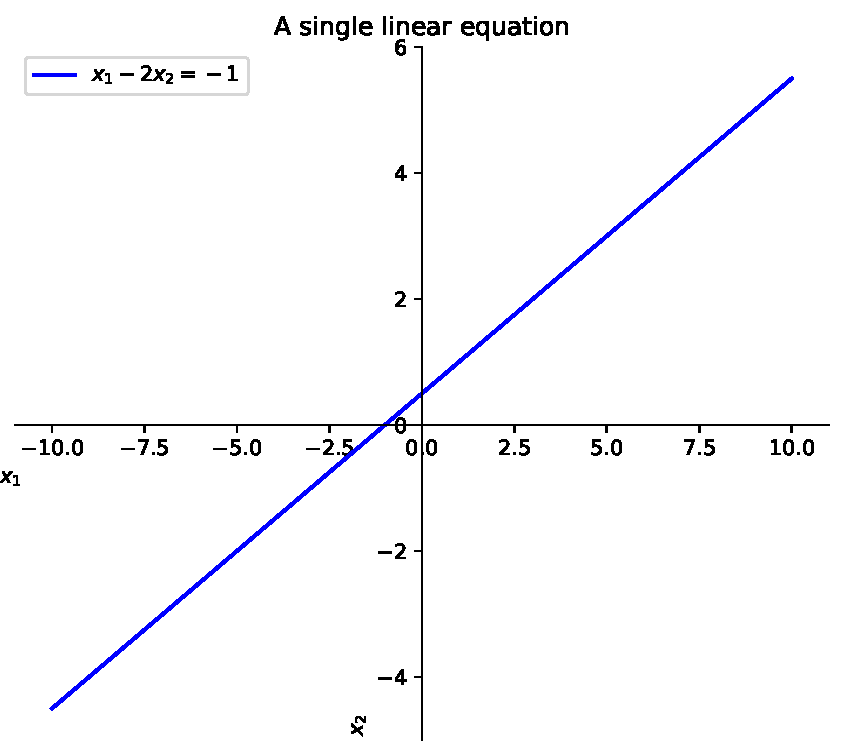
\includegraphics{p1_files/figure-pdf/cell-2-output-1.pdf}

}

\end{figure}

\begin{tcolorbox}[enhanced jigsaw, colbacktitle=quarto-callout-note-color!10!white, colback=white, colframe=quarto-callout-note-color-frame, title=\textcolor{quarto-callout-note-color}{\faInfo}\hspace{0.5em}{Definition of a linear equation}, opacityback=0, coltitle=black, left=2mm, leftrule=.75mm, rightrule=.15mm, opacitybacktitle=0.6, bottomrule=.15mm, titlerule=0mm, bottomtitle=1mm, breakable, toptitle=1mm, arc=.35mm, toprule=.15mm]

A linear equation in the variables \(x_1, x_2, \ldots, x_n\) is an
equation that can be written in the form

\[a_1x_1 + a_2x_2 + \cdots + a_nx_n = b\]

where \(b\) and the coefficients \(a_1, a_2, \ldots, a_n\) are real or
complex numbers. The subscript \(n\) may be any positive integer.

\end{tcolorbox}

Take the following \textbf{system of linear equations}: \[
\begin{align*}
x_1 - 2x_2 &= -1\\
-x_1 + 3x_2 &= 3
\end{align*}
\]

If we plot these equations on a graph, we can see that they intersect at
a single point. This point is the solution to the system of equations.

\begin{Shaded}
\begin{Highlighting}[]
\ImportTok{import}\NormalTok{ sympy }\ImportTok{as}\NormalTok{ sp}
\ImportTok{import}\NormalTok{ matplotlib.pyplot }\ImportTok{as}\NormalTok{ plt}
\ImportTok{import}\NormalTok{ numpy }\ImportTok{as}\NormalTok{ np}

\NormalTok{x1, x2 }\OperatorTok{=}\NormalTok{ sp.symbols(}\StringTok{\textquotesingle{}x\_1 x\_2\textquotesingle{}}\NormalTok{)}

\NormalTok{equation\_1 }\OperatorTok{=}\NormalTok{ sp.Eq(x1 }\OperatorTok{{-}} \DecValTok{2}\OperatorTok{*}\NormalTok{x2, }\OperatorTok{{-}}\DecValTok{1}\NormalTok{)}
\NormalTok{graph\_eq1 }\OperatorTok{=}\NormalTok{ sp.solve(equation\_1, x2)[}\DecValTok{0}\NormalTok{]}

\NormalTok{equation\_2 }\OperatorTok{=}\NormalTok{ sp.Eq(}\OperatorTok{{-}}\NormalTok{x1 }\OperatorTok{+} \DecValTok{3}\OperatorTok{*}\NormalTok{x2, }\DecValTok{3}\NormalTok{)}
\NormalTok{graph\_eq2 }\OperatorTok{=}\NormalTok{ sp.solve(equation\_2, x2)[}\DecValTok{0}\NormalTok{]}

\CommentTok{\# Generate data for plotting}
\NormalTok{x1\_vals }\OperatorTok{=}\NormalTok{ np.linspace(}\OperatorTok{{-}}\DecValTok{10}\NormalTok{, }\DecValTok{10}\NormalTok{, }\DecValTok{400}\NormalTok{)}
\NormalTok{graph\_eq1\_lambdified }\OperatorTok{=}\NormalTok{ sp.lambdify(x1, graph\_eq1)}
\NormalTok{graph\_eq2\_lambdified }\OperatorTok{=}\NormalTok{ sp.lambdify(x1, graph\_eq2)}
\NormalTok{y1\_vals }\OperatorTok{=}\NormalTok{ graph\_eq1\_lambdified(x1\_vals)}
\NormalTok{y2\_vals }\OperatorTok{=}\NormalTok{ graph\_eq2\_lambdified(x1\_vals)}

\CommentTok{\# Plotting}
\NormalTok{fig, ax }\OperatorTok{=}\NormalTok{ plt.subplots(figsize}\OperatorTok{=}\NormalTok{(}\DecValTok{7}\NormalTok{, }\DecValTok{6}\NormalTok{))}

\NormalTok{ax.set\_title(}\StringTok{\textquotesingle{}A system of equations with a single solution\textquotesingle{}}\NormalTok{)}
\NormalTok{ax.set\_xlabel(}\StringTok{\textquotesingle{}$x\_1$                                                                                                                            \textquotesingle{}}\NormalTok{)}
\NormalTok{ax.set\_ylabel(}\StringTok{\textquotesingle{}$x\_2$                                                                                                    \textquotesingle{}}\NormalTok{)}

\CommentTok{\# Plot the equations}
\NormalTok{ax.plot(x1\_vals, y1\_vals, label}\OperatorTok{=}\StringTok{\textquotesingle{}$x\_1 {-} 2x\_2 = {-}1$\textquotesingle{}}\NormalTok{, color}\OperatorTok{=}\StringTok{\textquotesingle{}blue\textquotesingle{}}\NormalTok{)}
\NormalTok{ax.plot(x1\_vals, y2\_vals, label}\OperatorTok{=}\StringTok{\textquotesingle{}${-}x\_1 + 3x\_2 = 3$\textquotesingle{}}\NormalTok{, color}\OperatorTok{=}\StringTok{\textquotesingle{}green\textquotesingle{}}\NormalTok{)}

\CommentTok{\# Move the left and bottom spines to x = 0 and y = 0, respectively}
\NormalTok{ax.spines[}\StringTok{\textquotesingle{}left\textquotesingle{}}\NormalTok{].set\_position(}\StringTok{\textquotesingle{}zero\textquotesingle{}}\NormalTok{)}
\NormalTok{ax.spines[}\StringTok{\textquotesingle{}bottom\textquotesingle{}}\NormalTok{].set\_position(}\StringTok{\textquotesingle{}zero\textquotesingle{}}\NormalTok{)}
\NormalTok{ax.spines[}\StringTok{\textquotesingle{}right\textquotesingle{}}\NormalTok{].set\_color(}\StringTok{\textquotesingle{}none\textquotesingle{}}\NormalTok{)}
\NormalTok{ax.spines[}\StringTok{\textquotesingle{}top\textquotesingle{}}\NormalTok{].set\_color(}\StringTok{\textquotesingle{}none\textquotesingle{}}\NormalTok{)}

\CommentTok{\# Add legend and grid}
\NormalTok{ax.legend()}
\NormalTok{plt.show()}
\end{Highlighting}
\end{Shaded}

\begin{figure}[H]

{\centering 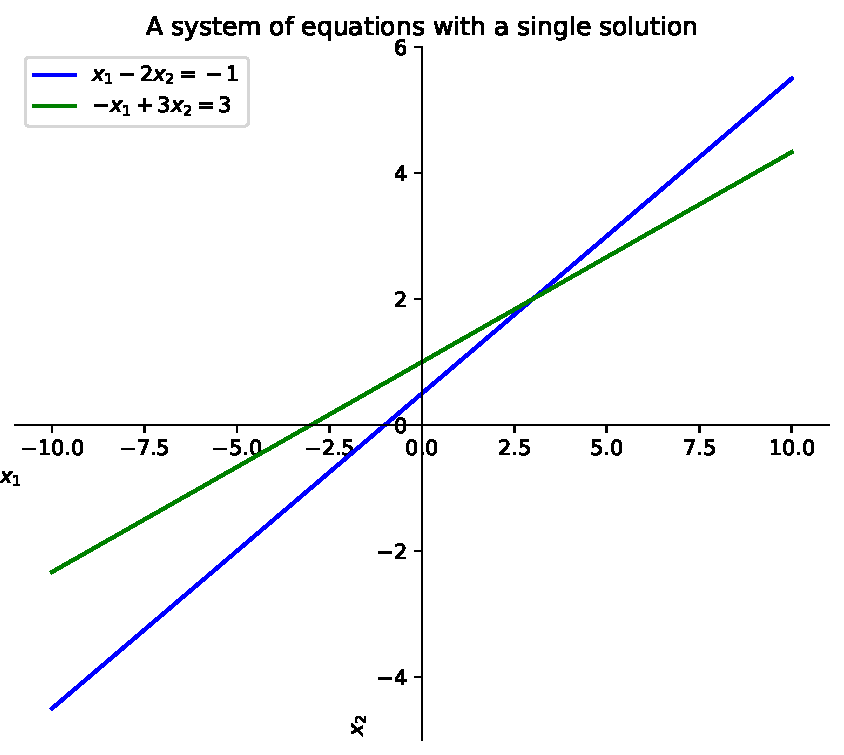
\includegraphics{p1_files/figure-pdf/cell-3-output-1.pdf}

}

\end{figure}

\begin{tcolorbox}[enhanced jigsaw, colbacktitle=quarto-callout-note-color!10!white, colback=white, colframe=quarto-callout-note-color-frame, title=\textcolor{quarto-callout-note-color}{\faInfo}\hspace{0.5em}{Definition of a system of linear equations}, opacityback=0, coltitle=black, left=2mm, leftrule=.75mm, rightrule=.15mm, opacitybacktitle=0.6, bottomrule=.15mm, titlerule=0mm, bottomtitle=1mm, breakable, toptitle=1mm, arc=.35mm, toprule=.15mm]

A system of linear equations (or a linear system) is a collection of one
or more linear equations involving the same variables- say
\(x_1, x_2, \ldots, x_n\). An example is

\[
\begin{align*}
x_1 - 2x_2 &= -1\\
-x_1 + 3x_2 &= 3
\end{align*}
\]

The above system has two equations and two variables where \(x_1, x_2\)
are the variables.

\end{tcolorbox}

The equations above have only one solution since they intersect at a
single point.

\begin{Shaded}
\begin{Highlighting}[]
\ImportTok{from}\NormalTok{ IPython.display }\ImportTok{import}\NormalTok{ Markdown}

\NormalTok{solution }\OperatorTok{=}\NormalTok{ sp.solve((equation\_1, equation\_2), (x1, x2))}
\NormalTok{Markdown(}\SpecialStringTok{f\textquotesingle{}$$}\CharTok{\textbackslash{}n}\SpecialCharTok{\{}\NormalTok{sp}\SpecialCharTok{.}\NormalTok{latex(solution)}\SpecialCharTok{\}}\CharTok{\textbackslash{}n}\SpecialStringTok{$$\textquotesingle{}}\NormalTok{)}
\end{Highlighting}
\end{Shaded}

\[
\left\{ x_{1} : 3, \  x_{2} : 2\right\}
\]

\begin{Shaded}
\begin{Highlighting}[]
\ImportTok{import}\NormalTok{ sympy }\ImportTok{as}\NormalTok{ sp}
\ImportTok{import}\NormalTok{ matplotlib.pyplot }\ImportTok{as}\NormalTok{ plt}
\ImportTok{import}\NormalTok{ numpy }\ImportTok{as}\NormalTok{ np}

\NormalTok{x1, x2 }\OperatorTok{=}\NormalTok{ sp.symbols(}\StringTok{\textquotesingle{}x\_1 x\_2\textquotesingle{}}\NormalTok{)}

\NormalTok{equation\_1 }\OperatorTok{=}\NormalTok{ sp.Eq(x1 }\OperatorTok{{-}} \DecValTok{2}\OperatorTok{*}\NormalTok{x2, }\OperatorTok{{-}}\DecValTok{1}\NormalTok{)}
\NormalTok{graph\_eq1 }\OperatorTok{=}\NormalTok{ sp.solve(equation\_1, x2)[}\DecValTok{0}\NormalTok{]}

\NormalTok{equation\_2 }\OperatorTok{=}\NormalTok{ sp.Eq(}\OperatorTok{{-}}\NormalTok{x1 }\OperatorTok{+} \DecValTok{3}\OperatorTok{*}\NormalTok{x2, }\DecValTok{3}\NormalTok{)}
\NormalTok{graph\_eq2 }\OperatorTok{=}\NormalTok{ sp.solve(equation\_2, x2)[}\DecValTok{0}\NormalTok{]}

\CommentTok{\# Generate data for plotting}
\NormalTok{x1\_vals }\OperatorTok{=}\NormalTok{ np.linspace(}\OperatorTok{{-}}\DecValTok{10}\NormalTok{, }\DecValTok{10}\NormalTok{, }\DecValTok{400}\NormalTok{)}
\NormalTok{graph\_eq1\_lambdified }\OperatorTok{=}\NormalTok{ sp.lambdify(x1, graph\_eq1)}
\NormalTok{graph\_eq2\_lambdified }\OperatorTok{=}\NormalTok{ sp.lambdify(x1, graph\_eq2)}
\NormalTok{y1\_vals }\OperatorTok{=}\NormalTok{ graph\_eq1\_lambdified(x1\_vals)}
\NormalTok{y2\_vals }\OperatorTok{=}\NormalTok{ graph\_eq2\_lambdified(x1\_vals)}

\CommentTok{\# Plotting}
\NormalTok{fig, ax }\OperatorTok{=}\NormalTok{ plt.subplots(figsize}\OperatorTok{=}\NormalTok{(}\DecValTok{7}\NormalTok{, }\DecValTok{6}\NormalTok{))}

\NormalTok{ax.set\_title(}\StringTok{\textquotesingle{}A system of equations with a single solution\textquotesingle{}}\NormalTok{)}
\NormalTok{ax.set\_xlabel(}\StringTok{\textquotesingle{}$x\_1$                                                                                                                            \textquotesingle{}}\NormalTok{)}
\NormalTok{ax.set\_ylabel(}\StringTok{\textquotesingle{}$x\_2$                                                                                                    \textquotesingle{}}\NormalTok{)}

\CommentTok{\# Plot the equations}
\NormalTok{ax.plot(x1\_vals, y1\_vals, label}\OperatorTok{=}\StringTok{\textquotesingle{}$x\_1 {-} 2x\_2 = {-}1$\textquotesingle{}}\NormalTok{, color}\OperatorTok{=}\StringTok{\textquotesingle{}blue\textquotesingle{}}\NormalTok{)}
\NormalTok{ax.plot(x1\_vals, y2\_vals, label}\OperatorTok{=}\StringTok{\textquotesingle{}${-}x\_1 + 3x\_2 = 3$\textquotesingle{}}\NormalTok{, color}\OperatorTok{=}\StringTok{\textquotesingle{}green\textquotesingle{}}\NormalTok{)}

\CommentTok{\# Move the left and bottom spines to x = 0 and y = 0, respectively}
\NormalTok{ax.spines[}\StringTok{\textquotesingle{}left\textquotesingle{}}\NormalTok{].set\_position(}\StringTok{\textquotesingle{}zero\textquotesingle{}}\NormalTok{)}
\NormalTok{ax.spines[}\StringTok{\textquotesingle{}bottom\textquotesingle{}}\NormalTok{].set\_position(}\StringTok{\textquotesingle{}zero\textquotesingle{}}\NormalTok{)}
\NormalTok{ax.spines[}\StringTok{\textquotesingle{}right\textquotesingle{}}\NormalTok{].set\_color(}\StringTok{\textquotesingle{}none\textquotesingle{}}\NormalTok{)}
\NormalTok{ax.spines[}\StringTok{\textquotesingle{}top\textquotesingle{}}\NormalTok{].set\_color(}\StringTok{\textquotesingle{}none\textquotesingle{}}\NormalTok{)}

\CommentTok{\# Plot the solution}
\NormalTok{solution }\OperatorTok{=}\NormalTok{ sp.solve((equation\_1, equation\_2), (x1, x2))}
\NormalTok{solution\_x1 }\OperatorTok{=}\NormalTok{ solution[x1]}
\NormalTok{solution\_x2 }\OperatorTok{=}\NormalTok{ solution[x2]}

\NormalTok{ax.scatter([solution\_x1], [solution\_x2], color}\OperatorTok{=}\StringTok{\textquotesingle{}red\textquotesingle{}}\NormalTok{, zorder}\OperatorTok{=}\DecValTok{3}\NormalTok{)  }
\NormalTok{ax.text(solution\_x1}\OperatorTok{+}\FloatTok{.5}\NormalTok{, solution\_x2}\OperatorTok{{-}}\FloatTok{.5}\NormalTok{, }\StringTok{\textquotesingle{}  Solution\textquotesingle{}}\NormalTok{, fontsize}\OperatorTok{=}\DecValTok{12}\NormalTok{)}

\CommentTok{\# Add legend and grid}
\NormalTok{ax.legend()}
\NormalTok{plt.show()}
\end{Highlighting}
\end{Shaded}

\begin{figure}[H]

{\centering 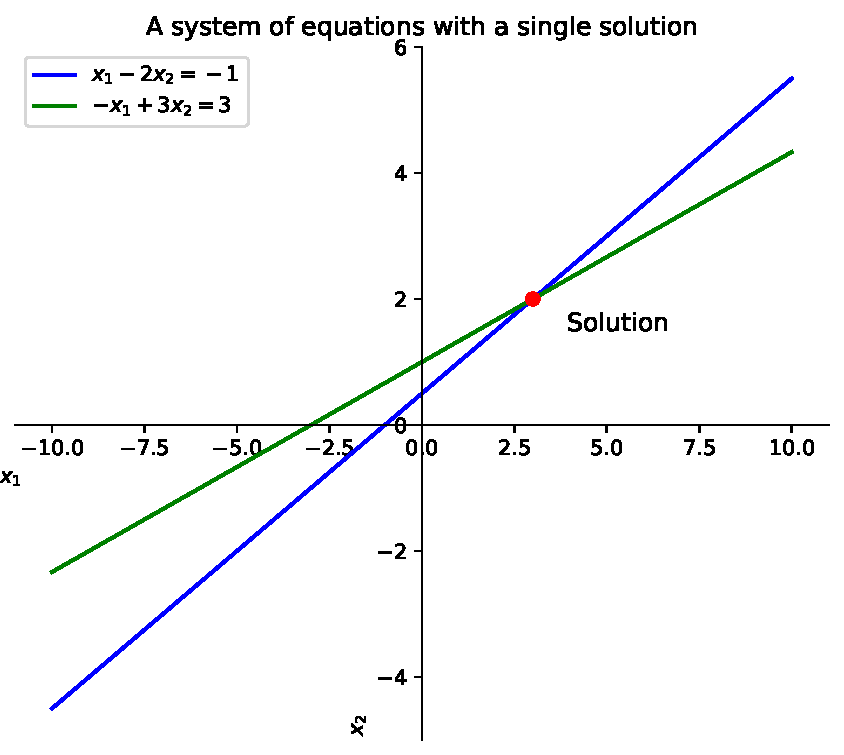
\includegraphics{p1_files/figure-pdf/cell-5-output-1.pdf}

}

\end{figure}

\begin{tcolorbox}[enhanced jigsaw, colbacktitle=quarto-callout-note-color!10!white, colback=white, colframe=quarto-callout-note-color-frame, title=\textcolor{quarto-callout-note-color}{\faInfo}\hspace{0.5em}{Definition of a solution}, opacityback=0, coltitle=black, left=2mm, leftrule=.75mm, rightrule=.15mm, opacitybacktitle=0.6, bottomrule=.15mm, titlerule=0mm, bottomtitle=1mm, breakable, toptitle=1mm, arc=.35mm, toprule=.15mm]

A solution of a linear system is a list of numbers
(\(s_1, s_2, \ldots, s_n\)) that makes each equation a true statement
when the values \(s_1, s_2, \ldots, s_n\) are substituted for
\(x_1, x_2, \ldots, x_n\), respectively.

For example, the list of numbers, \((3,2)\), is a solution of the system
above because, when the values \(3,2\) are substituted for \(x_1, x_2\),
respectively, both equations are a true statement.

\end{tcolorbox}

The above list, \((3,2)\), is the solution to the system of equations
because it is the only list of numbers that makes both equations true.
When we substitute \(3\) and \(2\) for \(x_1\) and \(x_2\) in the first
equation, both equations turn out to be true!

\[
\begin{align*}
x_1 - 2x_2 &= -1\\
-x_1 + 3x_2 &= 3
\end{align*}
\]

turns into

\[
\begin{align*}
(3) - 2(2) &= -1 \;\; &\text{True!}\\
-(3) + 3(2) &= 3 \;\; &\text{True!}
\end{align*}
\]

\hypertarget{systems-of-linear-equations-without-a-single-solution}{%
\section{Systems of Linear Equations without a Single
Solution}\label{systems-of-linear-equations-without-a-single-solution}}

\textbf{No Solution}

Take the following system of linear equations:

\[
\begin{align*}
x_1 - 2x_2 &= -1\\
-x_1 + 2x_2 &= 3
\end{align*}
\]

If we plot these equations on a graph, we can see that they are parallel
and never intersect. This means that there is no solution to this system
of equations.

\begin{Shaded}
\begin{Highlighting}[]
\ImportTok{import}\NormalTok{ sympy }\ImportTok{as}\NormalTok{ sp}
\ImportTok{import}\NormalTok{ matplotlib.pyplot }\ImportTok{as}\NormalTok{ plt}
\ImportTok{import}\NormalTok{ numpy }\ImportTok{as}\NormalTok{ np}

\NormalTok{x1, x2 }\OperatorTok{=}\NormalTok{ sp.symbols(}\StringTok{\textquotesingle{}x\_1 x\_2\textquotesingle{}}\NormalTok{)}

\CommentTok{\# Define the equations}
\NormalTok{equation\_1 }\OperatorTok{=}\NormalTok{ sp.Eq(x1 }\OperatorTok{{-}} \DecValTok{2}\OperatorTok{*}\NormalTok{x2, }\OperatorTok{{-}}\DecValTok{1}\NormalTok{)}
\NormalTok{graph\_eq1 }\OperatorTok{=}\NormalTok{ sp.solve(equation\_1, x2)[}\DecValTok{0}\NormalTok{]}

\NormalTok{equation\_2 }\OperatorTok{=}\NormalTok{ sp.Eq(}\OperatorTok{{-}}\NormalTok{x1 }\OperatorTok{+} \DecValTok{2}\OperatorTok{*}\NormalTok{x2, }\DecValTok{3}\NormalTok{)}
\NormalTok{graph\_eq2 }\OperatorTok{=}\NormalTok{ sp.solve(equation\_2, x2)[}\DecValTok{0}\NormalTok{]}

\CommentTok{\# Generate data for plotting}
\NormalTok{x1\_vals }\OperatorTok{=}\NormalTok{ np.linspace(}\OperatorTok{{-}}\DecValTok{10}\NormalTok{, }\DecValTok{10}\NormalTok{, }\DecValTok{400}\NormalTok{)}
\NormalTok{graph\_eq1\_lambdified }\OperatorTok{=}\NormalTok{ sp.lambdify(x1, graph\_eq1)}
\NormalTok{graph\_eq2\_lambdified }\OperatorTok{=}\NormalTok{ sp.lambdify(x1, graph\_eq2)}
\NormalTok{y1\_vals }\OperatorTok{=}\NormalTok{ graph\_eq1\_lambdified(x1\_vals)}
\NormalTok{y2\_vals }\OperatorTok{=}\NormalTok{ graph\_eq2\_lambdified(x1\_vals)}

\CommentTok{\# Plotting}
\NormalTok{fig, ax }\OperatorTok{=}\NormalTok{ plt.subplots(figsize}\OperatorTok{=}\NormalTok{(}\DecValTok{7}\NormalTok{, }\DecValTok{6}\NormalTok{))}

\NormalTok{ax.set\_title(}\StringTok{\textquotesingle{}A system of equations with no solution\textquotesingle{}}\NormalTok{)}
\NormalTok{ax.set\_xlabel(}\StringTok{\textquotesingle{}$x\_1$                                                                                                                            \textquotesingle{}}\NormalTok{)}
\NormalTok{ax.set\_ylabel(}\StringTok{\textquotesingle{}$x\_2$                                                                                                    \textquotesingle{}}\NormalTok{)}

\CommentTok{\# Plot the equations}
\NormalTok{ax.plot(x1\_vals, y1\_vals, label}\OperatorTok{=}\StringTok{\textquotesingle{}$x\_1 {-} 2x\_2 = {-}1$\textquotesingle{}}\NormalTok{, color}\OperatorTok{=}\StringTok{\textquotesingle{}blue\textquotesingle{}}\NormalTok{)}
\NormalTok{ax.plot(x1\_vals, y2\_vals, label}\OperatorTok{=}\StringTok{\textquotesingle{}${-}x\_1 + 2x\_2 = 3$\textquotesingle{}}\NormalTok{, color}\OperatorTok{=}\StringTok{\textquotesingle{}green\textquotesingle{}}\NormalTok{)}

\CommentTok{\# Move the left and bottom spines to x = 0 and y = 0, respectively}
\NormalTok{ax.spines[}\StringTok{\textquotesingle{}left\textquotesingle{}}\NormalTok{].set\_position(}\StringTok{\textquotesingle{}zero\textquotesingle{}}\NormalTok{)}
\NormalTok{ax.spines[}\StringTok{\textquotesingle{}bottom\textquotesingle{}}\NormalTok{].set\_position(}\StringTok{\textquotesingle{}zero\textquotesingle{}}\NormalTok{)}
\NormalTok{ax.spines[}\StringTok{\textquotesingle{}right\textquotesingle{}}\NormalTok{].set\_color(}\StringTok{\textquotesingle{}none\textquotesingle{}}\NormalTok{)}
\NormalTok{ax.spines[}\StringTok{\textquotesingle{}top\textquotesingle{}}\NormalTok{].set\_color(}\StringTok{\textquotesingle{}none\textquotesingle{}}\NormalTok{)}

\CommentTok{\# Add legend and grid}
\NormalTok{ax.legend()}
\NormalTok{plt.show()}
\end{Highlighting}
\end{Shaded}

\begin{figure}[H]

{\centering 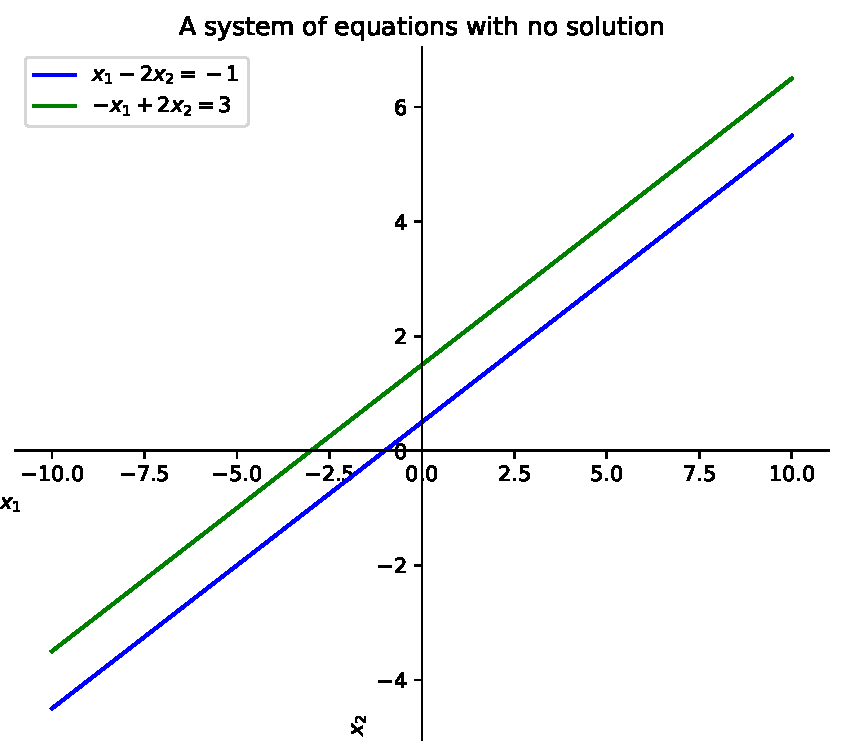
\includegraphics{p1_files/figure-pdf/cell-6-output-1.pdf}

}

\end{figure}

\textbf{Infinite Solutions}

Take the following system of linear equations:

\[
\begin{align*}
x_1 - 2x_2 &= -1\\
-x_1 + 2x_2 &= 1
\end{align*}
\]

If we plot these equations on a graph, we can see that they are the same
line. This means that there are an infinite number of solutions to this
system of equations.

\begin{Shaded}
\begin{Highlighting}[]
\ImportTok{import}\NormalTok{ sympy }\ImportTok{as}\NormalTok{ sp}
\ImportTok{import}\NormalTok{ matplotlib.pyplot }\ImportTok{as}\NormalTok{ plt}
\ImportTok{import}\NormalTok{ numpy }\ImportTok{as}\NormalTok{ np}

\NormalTok{x1, x2 }\OperatorTok{=}\NormalTok{ sp.symbols(}\StringTok{\textquotesingle{}x\_1 x\_2\textquotesingle{}}\NormalTok{)}

\CommentTok{\# Define the equations}
\NormalTok{equation\_1 }\OperatorTok{=}\NormalTok{ sp.Eq(x1 }\OperatorTok{{-}} \DecValTok{2}\OperatorTok{*}\NormalTok{x2, }\OperatorTok{{-}}\DecValTok{1}\NormalTok{)}
\NormalTok{graph\_eq1 }\OperatorTok{=}\NormalTok{ sp.solve(equation\_1, x2)[}\DecValTok{0}\NormalTok{]}

\NormalTok{equation\_2 }\OperatorTok{=}\NormalTok{ sp.Eq(}\OperatorTok{{-}}\NormalTok{x1 }\OperatorTok{+} \DecValTok{2}\OperatorTok{*}\NormalTok{x2, }\DecValTok{1}\NormalTok{)}
\NormalTok{graph\_eq2 }\OperatorTok{=}\NormalTok{ sp.solve(equation\_2, x2)[}\DecValTok{0}\NormalTok{]}

\CommentTok{\# Generate data for plotting}
\NormalTok{x1\_vals }\OperatorTok{=}\NormalTok{ np.linspace(}\OperatorTok{{-}}\DecValTok{10}\NormalTok{, }\DecValTok{10}\NormalTok{, }\DecValTok{400}\NormalTok{)}
\NormalTok{graph\_eq1\_lambdified }\OperatorTok{=}\NormalTok{ sp.lambdify(x1, graph\_eq1)}
\NormalTok{graph\_eq2\_lambdified }\OperatorTok{=}\NormalTok{ sp.lambdify(x1, graph\_eq2)}
\NormalTok{y1\_vals }\OperatorTok{=}\NormalTok{ graph\_eq1\_lambdified(x1\_vals)}
\NormalTok{y2\_vals }\OperatorTok{=}\NormalTok{ graph\_eq2\_lambdified(x1\_vals)}

\CommentTok{\# Plotting}
\NormalTok{fig, ax }\OperatorTok{=}\NormalTok{ plt.subplots(figsize}\OperatorTok{=}\NormalTok{(}\DecValTok{7}\NormalTok{, }\DecValTok{6}\NormalTok{))}

\NormalTok{ax.set\_title(}\StringTok{\textquotesingle{}A system of equations with infinite solutions\textquotesingle{}}\NormalTok{)}
\NormalTok{ax.set\_xlabel(}\StringTok{\textquotesingle{}$x\_1$                                                                                                                            \textquotesingle{}}\NormalTok{)}
\NormalTok{ax.set\_ylabel(}\StringTok{\textquotesingle{}$x\_2$                                                                                                    \textquotesingle{}}\NormalTok{)}

\CommentTok{\# Plot the equations}
\NormalTok{ax.plot(x1\_vals, y1\_vals, label}\OperatorTok{=}\StringTok{\textquotesingle{}$x\_1 {-} 2x\_2 = {-}1$\textquotesingle{}}\NormalTok{, color}\OperatorTok{=}\StringTok{\textquotesingle{}blue\textquotesingle{}}\NormalTok{)}
\NormalTok{ax.plot(x1\_vals, y2\_vals, label}\OperatorTok{=}\StringTok{\textquotesingle{}${-}x\_1 + 2x\_2 = 1$\textquotesingle{}}\NormalTok{, color}\OperatorTok{=}\StringTok{\textquotesingle{}green\textquotesingle{}}\NormalTok{, linestyle}\OperatorTok{=}\StringTok{\textquotesingle{}dashed\textquotesingle{}}\NormalTok{)}

\CommentTok{\# Move the left and bottom spines to x = 0 and y = 0, respectively}
\NormalTok{ax.spines[}\StringTok{\textquotesingle{}left\textquotesingle{}}\NormalTok{].set\_position(}\StringTok{\textquotesingle{}zero\textquotesingle{}}\NormalTok{)}
\NormalTok{ax.spines[}\StringTok{\textquotesingle{}bottom\textquotesingle{}}\NormalTok{].set\_position(}\StringTok{\textquotesingle{}zero\textquotesingle{}}\NormalTok{)}
\NormalTok{ax.spines[}\StringTok{\textquotesingle{}right\textquotesingle{}}\NormalTok{].set\_color(}\StringTok{\textquotesingle{}none\textquotesingle{}}\NormalTok{)}
\NormalTok{ax.spines[}\StringTok{\textquotesingle{}top\textquotesingle{}}\NormalTok{].set\_color(}\StringTok{\textquotesingle{}none\textquotesingle{}}\NormalTok{)}

\CommentTok{\# Add legend and grid}
\NormalTok{ax.legend()}
\NormalTok{plt.show()}
\end{Highlighting}
\end{Shaded}

\begin{figure}[H]

{\centering 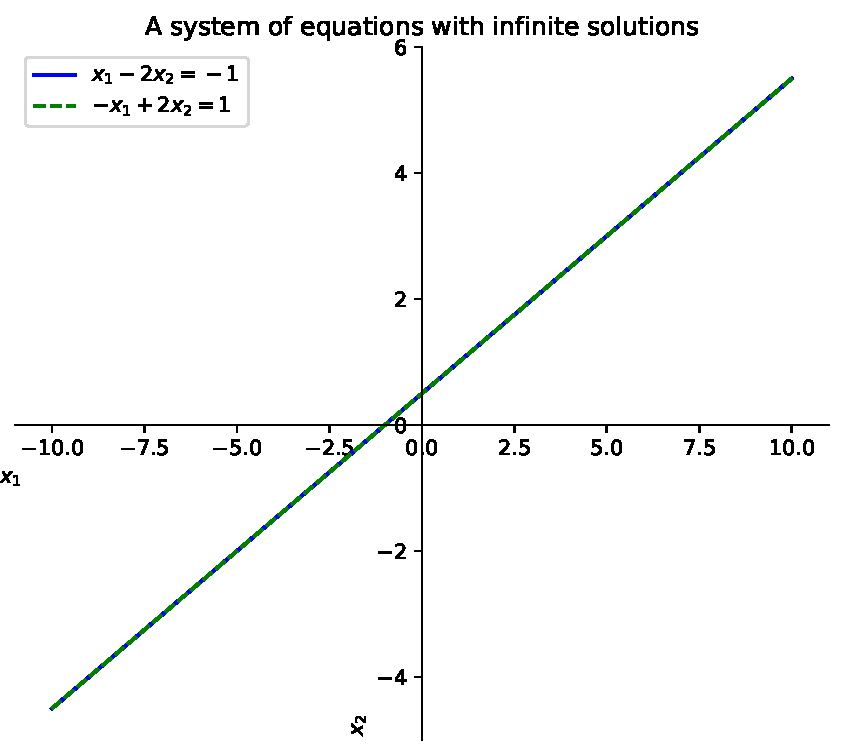
\includegraphics{p1_files/figure-pdf/cell-7-output-1.pdf}

}

\end{figure}

\begin{tcolorbox}[enhanced jigsaw, colbacktitle=quarto-callout-tip-color!10!white, colback=white, colframe=quarto-callout-tip-color-frame, title=\textcolor{quarto-callout-tip-color}{\faLightbulb}\hspace{0.5em}{Tip}, opacityback=0, coltitle=black, left=2mm, leftrule=.75mm, rightrule=.15mm, opacitybacktitle=0.6, bottomrule=.15mm, titlerule=0mm, bottomtitle=1mm, breakable, toptitle=1mm, arc=.35mm, toprule=.15mm]

A system of linear equations has

\begin{enumerate}
\def\labelenumi{\arabic{enumi}.}
\tightlist
\item
  no solution, or
\item
  exactly one solution, or
\item
  infinitely many solutions.
\end{enumerate}

\end{tcolorbox}

\bookmarksetup{startatroot}

\hypertarget{summary}{%
\chapter{Summary}\label{summary}}

In summary, this book has no content whatsoever.

\bookmarksetup{startatroot}

\hypertarget{references}{%
\chapter*{References}\label{references}}
\addcontentsline{toc}{chapter}{References}

\markboth{References}{References}

\hypertarget{refs}{}
\begin{CSLReferences}{0}{0}
\end{CSLReferences}



\end{document}
